\chapter{Semantic Analyses \& Typing} \label{chp:semantic-analyses}

\todobox{Overview and signposting paragraph}

\section{Typing AST and Desugaring} \label{sec:desugaring}

If the source program was successfully parsed to the parse AST representation of
\cref{fig:parse-ast}, we proceed by translating the parsed program to a new AST
representation used in the typing stage.
\cref{fig:type-ast} shows this new \emph{typing AST}.
As you can see, the definition has shrunk somewhat when compared to the AST of
the parsing stage. This is mostly due to the fact that all field selectors and
operators on expressions have been converted to regular function calls (case
\haskell{FunCallE}), although field selectors in variable assignments remain
unchanged.\todo{Mention how we keep them distinct}
In addition, all the garbage nodes available in the parse AST are no longer
present in the typing AST: since the garbage nodes indicate errors in the
parsing stage, we should not proceed to the typing stage in their presence.
The desugaring stage includes sanity checks that throw an error if such nodes
are found in the parsed program.

\begin{figure}
\begin{minted}[breaklines]{haskell}
data Program varAnn funAnn = Program [VarDecl varAnn] [FunMutDecl varAnn funAnn]
data VarDecl a = VarDecl Loc (Maybe UType) T.Text (Expr a) a
data FunDecl a b = FunDecl Loc T.Text [T.Text] (Maybe UType) [VarDecl a] [Stmt a] b
data FunMutDecl a b = MutualDecls Loc [FunDecl a b] | SingleDecl (FunDecl a b)

data Stmt a = If Loc (Expr a) [Stmt a] [Stmt a]
            | While Loc (Expr a) [Stmt a]
            | Assign Loc VarLookup a (Expr a)
            | FunCall Loc FunName [Expr a]
            | Return Loc (Maybe (Expr a))

data VarLookup = VarId Loc T.Text | VarField Loc VarLookup Field
data Field = Head | Tail | Fst | Snd

data FunName = Name T.Text
             | Not | Neg
             | Add | Sub | Mul | Div | Mod
             | Eq | Neq | Lt | Gt | Lte | Gte
             | And | Or
             | Cons | IsEmpty
             | HeadFun | TailFun | FstFun | SndFun
             | Print

data Expr a = Ident Loc T.Text a
            | Int Loc Int a
            | Char Loc Char a
            | Bool Loc Bool a
            | FunCallE Loc FunName [Expr a] a
            | EmptyList Loc a
            | Tuple Loc (Expr a) (Expr a) a

type UVar = Int
type TVar = T.Text

data UType = Int | Bool | Char | Void
           | Prod UType UType | List UType | Fun [UType] UType
           | UVar UVar | TVar TVar
\end{minted}

\caption{Abstract syntax tree for typing stage}
\label{fig:type-ast}
\end{figure}

Another key difference is that we extend many of the nodes with type
parameters \code{a} and \code{b}. The fields correspond to the types we
infer for the respective nodes during the typing stage.
Initially, we have no type information available (aside from the optional type
annotations in the source program), and represent this lack of information
with the \haskell{()} type, e.g. \haskell{Expr ()}. During the typing stage, we
iterate through the typing AST, replacing these dummy fields of type \haskell{()}
with our inferred type information, represented by \haskell{UType}.
For instance, when checking an expression $e$, we start with an instance of
\haskell{Expr ()}, and return an instance of \haskell{Expr UType}.
The definition of \haskell{UType} is also given in \cref{fig:type-ast}, and
corresponds to the grammar of SPL types, with the addition of \emph{unification
variables} \haskell{UVar}.\todo{Point out \haskell{MutualDecls} node}
Unification variables are represented simply by integers, and are generated as
placeholders for unknown types during type checking. While iterating through the
AST, we annotate the nodes with these unification variables, and simultaneously
generate a set of constraints between them, expressing how the (currently still
unknown) types must relate to each other.\todo{Fix this description}

\todobox{Which nodes feature type information, and which just `thread through' the
type parameters?}

To illustrate, let us consider a simple example: say we are typing the
expression \spl{(1,2).fst}. The field selector \spl{.fst} will be desugared
to a regular function, meaning we can think of the expression as something
closer to \spl{fstfun((1,2))}. The type of \spl{fstfun} is polymorphic, and
given by $\forall \alpha \beta.\ (\alpha,\beta) \to \alpha$, expressing that
from a tuple with entries of type $\alpha$ and $\beta$ (respectively),
\spl{fstfun} returns the first entry with type $\alpha$.
During typing, we generate unification variables $\alpha_1$, $\alpha_2$ and
$\beta$, where $(\alpha_1,\alpha_2)$ is the input type of \spl{fstfun}, $\beta$
is the output type and thus the type of \spl{(1,true).fst}, and we also know
that $\alpha_1 = \beta$, since we are selecting the first component.
Next, we look at the pair constructor, whose type is given as the \emph{product}
of the two inner types, that is, the types of \spl{1} and \spl{true}.
These, in turn, are trivial to typecheck, and do not yield any constraints or
substitutions. Given that \spl{(1,true)} has type \spl{(Int,Bool)}, we return
to the constraints from earlier:
We now know that \code{($\alpha_1$,$\alpha_2$) $=$ (Int,Bool)}, so by
$\alpha_1 = \beta$ we conclude that \spl{(1,true).fst} has type
$\beta = \code{Int}$.

% \begin{figure}
% \begin{minted}[breaklines]{haskell}
% type UVar = Int
% type TVar = T.Text

% data UType = Int | Bool | Char | Void
%            | Prod UType UType | List UType | Fun [UType] UType
%            | UVar UVar | TVar TVar
% \end{minted}

%   \caption{Algebraic data type of SPL types}
%   \label{fig:type-adt}
% \end{figure}


\section{SCC Analysis}

In a function declaration---represented by \haskell{FunDecl a b} in the
AST representation of \cref{fig:type-ast}---the body may freely contain function
calls to other functions, as well as the function itself.
In the typing algorithm, we must ensure that we process function declarations in
the right order, based on how they reference each other.
If the declaration for some function $f$ refers to a function $g$, we need to
process $g$ first, since we need its type to check that $g$ is used correctly in
the body of $f$.

While we could simply require that the user declare a function before other
functions that reference it, we are able to statically infer this ordering using
the \emph{call graph} of the program.
The call graph has as its nodes the functions declared in the program, while the
edges are given by the function calls between them: if some function $f$ calls
the function $g$, this is captured by a directed edge from $f$ to $g$.

There is also the possibility that a function refers to itself
(\emph{recursion}), and---more importantly---that two or more functions refer to
each other in a cycle, in which case they are said to be \emph{mutually
recursive}. We want to identify such groups of functions, since we need some
additional steps in the typing algorithm to handle them correctly.
Again, we can leverage the call graph to find groups of nodes that refer to each
other cyclically; in graph terminology, these are referred to as
\emph{strongly connected components} (SCCs).
Our overall goal is thus to construct the call graph of the input program and
use it to find the SCCs, as well as sorting the (groups of) functions such that
they appear in the output prior to the functions that refer to them.
More formally, we want the reverse \emph{topological} sorting of the directed
acyclic graph given by the SCCs of the original call graph.

The so-called strongly connected components algorithm of \citet{Tarjan1972}
lends itself very elegantly to this problem, as it identifies the SCCs of a
directed graph in linear time, while also returning the SCCs in reverse
topological ordering as a by-product.
We do not discuss the inner workings of the algorithm, and our compiler uses an
existing Haskell implementation of Tarjan's algorithm provided in the
\code{Data.Graph} library, based on the algorithm description of
\citet{King1995}.

\paragraph{Call graph generation}
In order to use the library implementation of the SCC algorithm, we must
construct the call graph for the input program in the appropriate format for the
library function, and then process the output back into our AST representation,
which gives us the sorted program.
We generate the call graph using the following monad:
\begin{minted}{haskell}
  type GraphGen = StateT GraphGenState (Except T.Text)
\end{minted}
%
Generating the graph requires some auxiliary data structures, which we thread
through the computation using the state monad, where the state is given by
\haskell{GraphGenState}\footnote{We define type aliases for the map types in our
implementation. \haskell{Vertex} is a synonym for \haskell{Int}.}:
\begin{minted}{haskell}
  data GraphGenState = GraphGenState {
    nameMap  :: M.Map Name Vertex,
    declMap  :: M.Map Vertex (FunDecl () ()),
    edgeMap  :: M.Map Vertex (S.Set Vertex),
    vtxBound :: Vertex
  }
\end{minted}




\begin{figure}[h]

  \centering

  \begin{minipage}{.45\textwidth}
    \begin{lstlisting}[language=SPL]
      p(x) { $...$ }

      f(x) {
        $...$ g(x,x-1) $...$ p(x) $...$
      }

      g(x,y) {
        $...$ p(y) $...$ h(y) $...$
      }

      h(n) { $...$ f(n/2) $...$ g(n) $...$ }

      main() { var a = h(f(42)); $...$ }
    \end{lstlisting}
  \end{minipage}\hspace{6mm}%
  %
  \begin{minipage}{.45\textwidth}
    \begin{center}
      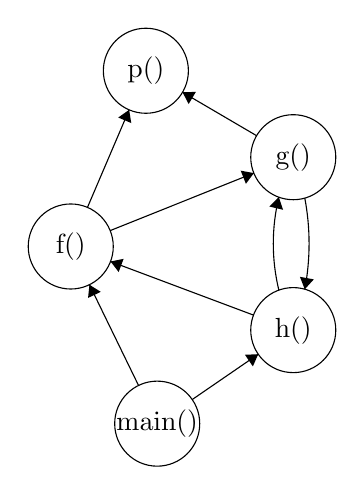
\begin{tikzpicture}[scale=0.18]
        \tikzstyle{every node}+=[inner sep=0pt]
        \draw [black] (33.9,-17.3) circle (3);
        \draw (33.9,-17.3) node { \code{p()} };
        \draw [black] (28.6,-29.7) circle (3);
        \draw (28.6,-29.7) node { \code{f()} };
        \draw [black] (44.3,-23.4) circle (3);
        \draw (44.3,-23.4) node { \code{g()} };
        \draw [black] (44.3,-35.6) circle (3);
        \draw (44.3,-35.6) node { \code{h()} };
        \draw [black] (34.7,-42.2) circle (3);
        \draw (34.7,-42.2) node { \code{main()} };
        \draw [black] (43.284,-32.784) arc (-166.34085:-193.65915:13.905);
        \fill [black] (43.28,-26.22) -- (42.61,-26.88) -- (43.58,-27.11);
        \draw [black] (45.113,-26.284) arc (10.75824:-10.75824:17.23);
        \fill [black] (45.11,-32.72) -- (45.75,-32.02) -- (44.77,-31.84);
        \draw [black] (31.38,-28.58) -- (41.52,-24.52);
        \fill [black] (41.52,-24.52) -- (40.59,-24.35) -- (40.96,-25.28);
        \draw [black] (41.49,-34.54) -- (31.41,-30.76);
        \fill [black] (31.41,-30.76) -- (31.98,-31.5) -- (32.33,-30.57);
        \draw [black] (41.71,-21.88) -- (36.49,-18.82);
        \fill [black] (36.49,-18.82) -- (36.92,-19.65) -- (37.43,-18.79);
        \draw [black] (29.78,-26.94) -- (32.72,-20.06);
        \fill [black] (32.72,-20.06) -- (31.95,-20.6) -- (32.87,-20.99);
        \draw [black] (37.17,-40.5) -- (41.83,-37.3);
        \fill [black] (41.83,-37.3) -- (40.89,-37.34) -- (41.45,-38.16);
        \draw [black] (33.38,-39.5) -- (29.92,-32.4);
        \fill [black] (29.92,-32.4) -- (29.82,-33.33) -- (30.72,-32.9);
      \end{tikzpicture}
    \end{center}
    \vspace{2mm}
  \end{minipage}

  \caption{Example program outline and corresponding call graph}

\end{figure}


\todobox{Briefly describe how we construct a graph of the function declarations,
how we use the SCC library function to get the topological sorting, and how we
convert the result back into a \haskell{Program} instance.}


\section{Scoping}
As specified in the grammar given in \cref{chp:grammar}, SPL only allows
variable declarations at the global level, or at the beginning of a function
body. SPL thus features only two scope levels: one global scope which covers
top-level variable definitions and all function declarations, and a local scope
per function, which features the function arguments and the local variables
declared at the start of the function body.

Consider the following example program:
%
\begin{lstlisting}[language=SPL]
  Int a = 2;

  main(x) :: -> Void {
    Int b = 20;
    print(b * x + a);
    return;
  }
\end{lstlisting}
%
Here, \spl{a} and \spl{f} are bound in the global scope, while \spl{x} and
\spl{b} are bound only in the body of function \spl{f}.

To represent this information, our type inference implementation uses two
variants of identifier, as well as two separate environments, one of which
stores global identifiers, while they other tracks local bindings.

\begin{minted}{haskell}
data LocalId = LocalTermVar T.Text | LocalFunName T.Text | RetType
data GlobalId = GlobalTermVar T.Text | GlobalFunName T.Text

data EnvLevel = GlobalLevel | LocalLevel

type GlobalEnv = M.Map GlobalId UScheme
type LocalEnv = M.Map LocalId UType
\end{minted}

The \haskell{LocalId} and \haskell{GlobalId} data types both distinguish between
term variables $x$ and function names $f$ at the respective levels.
\haskell{LocalId} additionally features the special case of \haskell{RetType},
which is used within the local scope of a function body to identify the return
type, as it has no explicit identifier in the source.
Next, we have \haskell{EnvLevel}, which simply serves as a toggle for certain
functions whose behaviour differs depending on the scope.
Finally, \haskell{GlobalEnv} maps \haskell{GlobalId}s to \haskell{UScheme}s,
while \haskell{LocalEnv} maps \haskell{LocalId}s to \haskell{UType}s.
The reason for using \haskell{UScheme} at the top level is that the types of
functions are generalised in the free unification variables, that is, they have
the general form $\forall\ \set{\alpha}.\ \tau$, while variables are always
assigned monotypes.


\section{Variables and Substitutions}

During the typing procedure, we must generate fresh unification variables and
work with substitutions, which we also need to compose and apply to types.
For generating fresh variable names, we simply keep track of an integer
\code{varState} under the state monad, which allows us to simply read and
increment the counter whenever we need a new name. Since the counter strictly
increases, we are guaranteed to obtain a (currently) unused name.

Substitutions $S$ are represented by maps from unification variables
\haskell{UVar} to (unification) types \haskell{UType}. Their type \haskell{Subst}
constitutes an instance of Haskell's \haskell{Monoid} typeclass, where the
binary operation is defined as composition $S_1 \circ S_2$, and the unit element
is given by the empty substitution $\emptyset$.

\begin{minted}{haskell}
instance Semigroup Subst where
  Subst s1 <> Subst s2 = Subst $ M.map (subst (Subst s1)) s2 `M.union` s1

instance Monoid Subst where
  mempty = Subst M.empty
\end{minted}

We write $\tau.S$ for applying the substitution $S$ to type $\tau$, where the
substitution procedure is defined as follows:

\[
\begin{array}{rcl}
  \alpha.S & \eqdef & S(\alpha) \\
  \Int.S & \eqdef & \Int \\
  \Bool.S & \eqdef & \Bool \\
  \Char.S & \eqdef & \Char \\
  \Void.S & \eqdef & \Void \\
  \TProd{\tau_1}{\tau_2}.S & \eqdef & \TProd{\tau_1.S}{\tau_2.S} \\
  \TList{\tau}.S & \eqdef & \TList{\tau.S} \br
  \Parens{ \TFun{\set{\sigma_i}}{\tau} }.S & \eqdef & \TFun{\set{\sigma_i.S}}{\tau.S}
\end{array}
\]

For the free (unification) variables in a type $\tau$, we write $\FV(\tau)$, where
$\FV(-)$ is defined by:

\[
\begin{array}{rcl}
  \FV(\alpha) & \eqdef & \{ \alpha \} \\
  \FV(\Int) & \eqdef & \emptyset \\
  \FV(\Bool) & \eqdef & \emptyset \\
  \FV(\Char) & \eqdef & \emptyset \\
  \FV(\Void) & \eqdef & \emptyset \\
  \FV( \TProd{\tau_1}{\tau_2} ) & \eqdef & \FV(\tau_1) \cup \FV(\tau_2) \\
  \FV( \TList{\tau} ) & \eqdef & \FV(\tau) \\
  \FV( \TFun{\set{\sigma_i}}{\tau} ) & \eqdef & \{ \FV(\sigma_i) \mid i \} \cup \FV(\tau)
\end{array}
\]

The operation $\unify$ takes two types and attempts to unify them, resulting in
a substitution $S$.

\[
\begin{array}{rcl}
  \unify(\Int,\Int) & \eqdef & \emptyset \\
  \unify(\Bool,\Bool) & \eqdef & \emptyset \\
  \unify(\Char,\Char) & \eqdef & \emptyset \\
  \unify(\Void,\Void) & \eqdef & \emptyset \\
  \unify(\alpha,\alpha) & \eqdef & \emptyset \\
  \unify(\alpha,\tau) & \eqdef &
    \{ \alpha \mapsto \tau \},\ \text{if}\ \alpha \notin \FV(\tau) \\
  \unify(\tau,\alpha) & \eqdef & \unify(\alpha,\tau) \\
  \unify(\TList{\tau},\TList{\sigma}) & \eqdef & \unify(\tau,\sigma)
  % \unify(\TProd{\tau_1}{\tau_2}, \TProd{\sigma_1}{\sigma_2}) & \eqdef &
\end{array}
\]

For all other combinations of types $\tau$ and $\sigma$ not covered by the
equations above, the types cannot be unified and the result of
$\unify(\tau,\sigma)$ is `\textsf{Fail}'.


\section{Typing Algorithm}

We now present our type inference algorithm. By misuse of notation, we describe
the cases of the algorithm in deduction rules, where the judgement
$\Gamma \vdash_W e : \tau, S$ states that in context $\Gamma$, the expression $e$
is typed with $\tau$ under generation of the substitution $S$.
When considering a list of expressions, such as the arguments to a function, we
use the overlined notation $\set{e_i}$ for $e_1,\dots,e_n$. Similarly, we
extend this notation to types, substitutions and the typing judgement, as seen
in e.g. \ruleref{W-FunCall}, where the judgement
\[ \set{ \Gamma \vdash_W e_i : \tau_i,\ S_i } \]
states that in context $\Gamma$, the $i$-th expression $e_i$ has type $\tau_i$,
generating the substitution $S_i$. We then write $\set{S_i}$ to mean the
composition of all $S_i$ in order, that is, $S_n \circ \dots \circ S_1$.
The judgement $\fresh(\alpha)$ states that the unification variable $\alpha$ is
freshly generated. We write $\inst(\forall\ \set{\alpha}.\ \tau)$ for the
typing scheme $\forall\ \set{\alpha}.\ \tau$ where all $\set{\alpha}$ are
substituted with fresh unification variables.
Finally, $\unify(\sigma,\tau)$ denotes the substitution generated by performing
the unification procedure on types $\sigma$ and $\tau$.

\begin{figure}[h]
  \begin{mathpar}

    \inferrule[W-Var]
      {\Gamma(x) = \tau}
      {\Gamma \vdash_W x : \tau,\ \emptyset}

    \inferrule[W-Int]{ }
      {\Gamma \vdash_W n : \code{Int},\ \emptyset}

    \inferrule[W-Bool]{ }
      {\Gamma \vdash_W b : \code{Bool},\ \emptyset}

    \inferrule[W-Char]{ }
      {\Gamma \vdash_W c : \code{Char},\ \emptyset}

    \inferrule[W-Empty]%
      {\fresh(\alpha)}
      {\Gamma \vdash_W \code{[]} : \code{[$\alpha$]},\ \emptyset}

    \inferrule[W-Tuple]%
      {\Gamma \vdash_W e_1 : \tau_1,\ S_1 \\
      \Gamma \vdash_W e_2 : \tau_2,\ S_2}
      {\Gamma \vdash_W \code{($e_1$,$e_2$)} : \code{($\tau_1$,$\tau_2$)},\ S_2 \circ S_1}

    \inferH{W-FunCall}%
      {\set{\sigma_i} \to \sigma = \mathit{inst}(\Gamma(f)) \\
        \set{ \Gamma \vdash_W e_i : \tau_i,\ S_i} \\
        S = \mathit{unify}(\set{\sigma_i, \tau_i})}
      {\Gamma \vdash_W \code{$f$($\set{e_i}$)} : \tau.S,\ S \circ \set{S_i}}
  \end{mathpar}

  \caption{Rules for the type inference algorithm on expressions}
  \label{fig:typing-rules-expr}
\end{figure}

\todobox{Figure out how to present type inference procedure on statements and
declarations, and add the corresponding rules.}

\todobox{Define unification procedure, and how the substitution is generated,
including lifting the unification to two lists of types, like when unifying
function arguments.}


\begin{todoenv}
  \begin{itemize}
    \item New Abstract Syntax Tree? Decorate existing Abstract Syntax Tree?
    \item Error messages?
    \item Polymorphism? Inference? Overloading?
    \item Problems?
    \item\ldots
  \end{itemize}
\end{todoenv}
